Singleton Interface method is based on fitting of all the parameters and customizations into single method definition.
Usually some of the parameters are nullable because there is some default value that is used in case
of the null value (specified in the business logic) or the parameter is not used at all in combination
with other parameters (for example, maximum response time is not used in case of the Leave Group message).
It is the simplest approach that can be used for designing of the API\@.

The Figure~\ref{fig:sing_write_igmp_packet} shows the activity diagram with interface definition of the
method for writing of the IGMPv2 packet into the output stream.
All parameters including type of the message are squashed into the single interface method.
Only parameters \textit{igmpType} and \textit{outputStream} are mandatory, other parameters may contain null values
depending on the value of \textit{igmpType} parameter.

\begin{figure}[!htb]
    \centering
    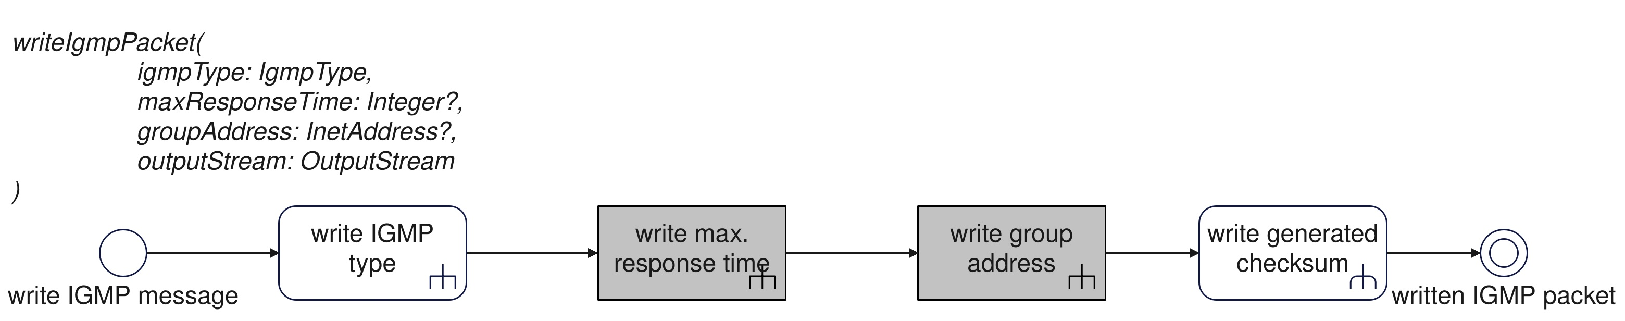
\includegraphics[width=1.0
    \textwidth]{sing_write_igmp_packet}
    \caption{Singleton Interface Method: Writing IGMP packet using }
    \label{fig:sing_write_igmp_packet}
\end{figure}

Activity diagram also contains more complex activities (write maximum response time and write group address)
that must be decomposed into the smaller diagrams.
For example, content of the write maximum response time activity is depicted
in the Figure~\ref{fig:sing_write_max_response_time}.
Since the whole logic is implemented under common interface method, the business logic contains a lot of branching
including conditional statements that are used for handling invalid combinations of the input parameters.

\begin{figure}[!htb]
    \centering
    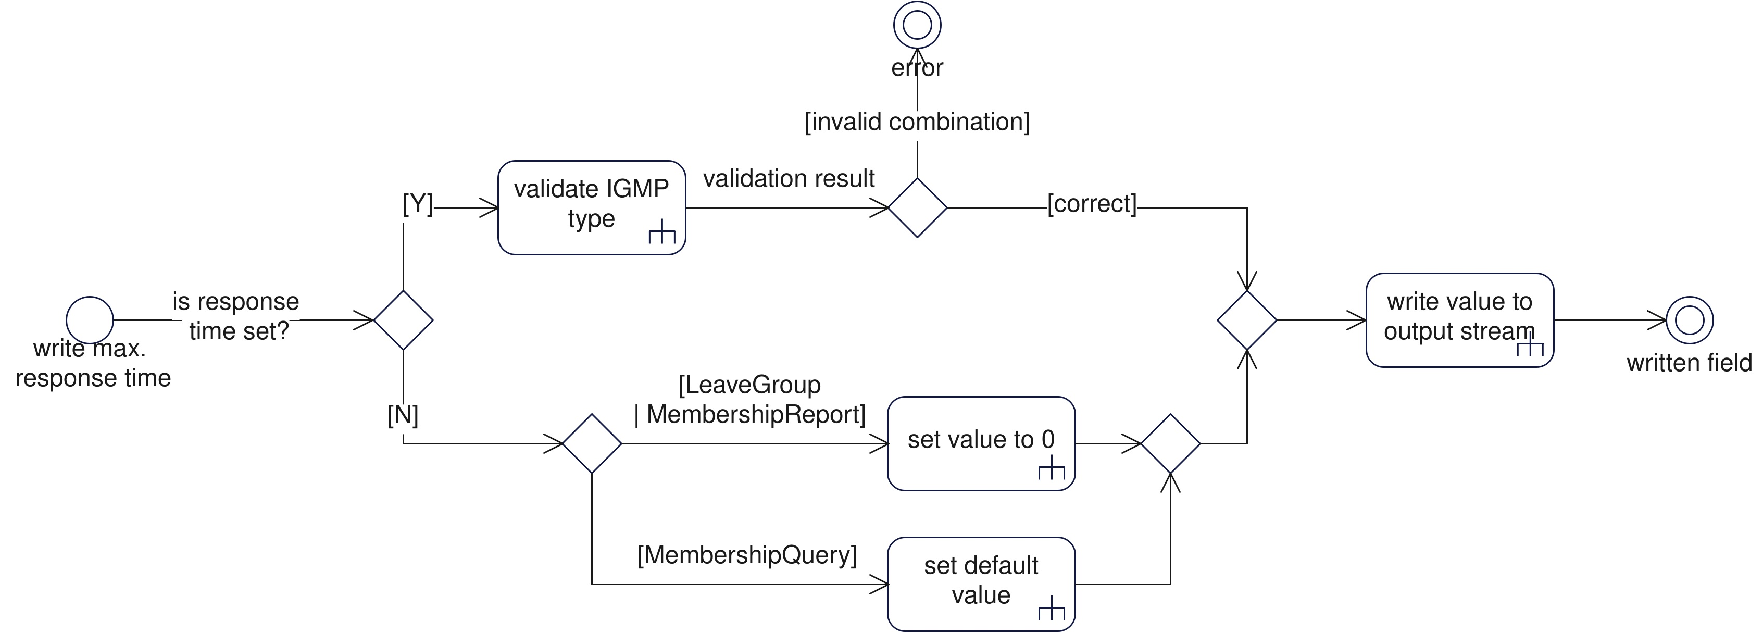
\includegraphics[width=1.0
    \textwidth]{sing_write_max_response_time}
    \caption{Singleton Interface Method: Writing maximum response time}
    \label{fig:sing_write_max_response_time}
\end{figure}

Benefits of the Singleton Interface Method:

\begin{itemize}
    \item Implementation of the interface is straightforward and simple.
    There is no need to implement any additional software entities.
    \item Single point of the contact for the API client may be beneficial in some cases.
    For example, client may represent just some additional proxy layer on top of the API that
    already receives all the required parameters from the other components in the system.
    Further decomposition of the layer would introduce unnecessary complexity in the proxy layer
    (calling correct method exposed by service based on some conditions).
\end{itemize}

Drawbacks of the Singleton Interface Method:

\begin{itemize}
    \item Appearance of God Classes/Functions - All the logic is implemented in single method which is usually
    very complex with a lot of branching.
    It is usually difficult to understand the logic and maintain it in the future.
    \item Evolution of the API is very hard - Supporting next packet fields, for example in case of the IGMPv3,
    would require to change the interface method signature and all the clients that are using it.
    \item Nullable parameters - Some of the parameters are nullable depending on the type of the IGMP message.
    Implementation must contain additional logic for handling of the invalid combinations of the parameters
    and client must be aware of the valid combinations.
    Additionally, default values that override null values are not transparent to client and must be explicitly
    documented.
    \item Long list of parameters is error-prone.
    If used technology does not support named parameters, client must be aware of the ordering.
    \item Violation of the Single Responsibility Principle (SRP) - Such methods tends to grow over time
    and usually contain more than one responsibility.
\end{itemize}

Common use-cases of the Singleton Interface Method:

\begin{itemize}
    \item Stable API that is not expected to change in the future,
    and it does not contain complex branching in the implementation.
    There is just single behaviour that is implemented by the service without customizations or subtypes.
    \item Simple services or utility functions with small number of non-null parameters.
\end{itemize}
